\documentclass[12pt,a4paper]{article}
\usepackage[a4paper,top=12mm,bottom=14mm,left=15mm,right=15mm]{geometry}
\usepackage[T1]{fontenc}
\usepackage{amsmath}
\usepackage{amssymb}
\usepackage{enumitem}
\usepackage{multicol}
\usepackage{array}
\usepackage{xcolor}
\usepackage{tikz}
\usepackage[most]{tcolorbox}
\usetikzlibrary{arrows.meta}

% ================================================================
% An introduction to surds.
%
% A first sheet on surds for a lower ability Year 10 class, designed
% to be worked through with the calculator on the desk. Surds are
% met first as square roots whose decimals never end. Pupils then
% work out a mixed list of surds and multiples of surds on the
% calculator and spot which of them are equal, which leads into the
% rule for simplifying surds. Adding and subtracting surds is built
% on collecting like terms in algebra, and multiplying and dividing
% surds is taught straight from the formulas, with the formulas for
% each part boxed. The sheet ends with "many ways to make a surd"
% diagrams: one worked example, then diagrams with less and less
% filled in. Answers are on the last page.
%
% The sheet is written on, so every question is followed by a
% working area. The \newpage commands in the body are placed so that
% no question is split across the fold.
% ================================================================

\pagestyle{empty}
\linespread{1.15}\selectfont
\setlength{\parskip}{5pt}
\setlist[enumerate,1]{label=\textbf{Q\arabic*.}, leftmargin=*, itemsep=10pt, topsep=6pt, parsep=4pt}
\setlist[enumerate,2]{label=(\alph*), leftmargin=*, itemsep=8pt, topsep=5pt, parsep=3pt}
\setlength{\multicolsep}{4pt}
\setlength{\parindent}{0pt}

\newcommand{\ansline}[1][2.2cm]{\underline{\hspace{#1}}}
% A short gap for a single number, sized to sit inside a line of maths.
\newcommand{\gap}{\underline{\hspace{0.7cm}}}
% A gap under a root sign. An underline leaves too little room beneath the
% radical, so a faint dotted box marks where the number is written instead.
% The box is the tallest that still keeps the ordinary-sized root sign,
% and is measured in em so that it scales with the type around it.
\newcommand{\rootgap}{\tikz[baseline=0pt]\draw[gray!60,densely dotted,thick]
  (0,-0.12em) rectangle (1.8em,0.83em);}

% A worked example: the method shown in full before it is practised.
% The boxes are tinted only faintly, and their title bars are pale with
% coloured text rather than solid, so that the sheet is cheap to print.
\newtcolorbox{wex}[1]{colback=blue!1,colframe=blue!45!black,boxrule=0.6pt,
  colbacktitle=blue!8,coltitle=blue!50!black,
  left=6pt,right=6pt,top=4pt,bottom=5pt,
  title={\bfseries\small Worked example: #1},fonttitle=\small,
  toptitle=1pt,bottomtitle=1pt}

% The idea a section is built on, stated once and boxed.
\newtcolorbox{keyidea}{colback=orange!2,colframe=orange!60!black,boxrule=0.6pt,
  left=6pt,right=6pt,top=4pt,bottom=4pt}

% The formulas for a section, set large so that they can be found
% again from anywhere on the sheet.
\newtcolorbox{formulas}[1]{colback=green!1,colframe=green!35!black,boxrule=0.9pt,
  colbacktitle=green!10,coltitle=green!30!black,
  left=8pt,right=8pt,top=5pt,bottom=5pt,
  title={\bfseries Formulas: #1},fonttitle=\normalsize,
  toptitle=2pt,bottomtitle=2pt}

% A warning about a mistake that is easy to make.
\newtcolorbox{warning}{colback=red!2,colframe=red!55!black,boxrule=0.6pt,
  left=6pt,right=6pt,top=4pt,bottom=4pt}

% The section headings, kept tight so the parts do not eat the page.
\newcommand{\heading}[1]{%
  \vspace{2pt}
  {\color{blue!45!black}\rule{\linewidth}{1pt}}\\[1pt]
  {\large\bfseries #1}\\[-6pt]
  {\color{blue!45!black}\rule{\linewidth}{0.4pt}}
  \vspace{2pt}}
\newcommand{\parttitle}[2]{\heading{Part #1: #2}}

% ----------------------------------------------------------------
% Calculator keys and screens, drawn to look like the keys pupils
% press. \calckey is a function key, \numkey a number key, and
% \calcscreen{<what was typed>}{<the answer shown>} a display.
\tikzset{fnkey/.style={draw=black!75,fill=black!75,text=white,rounded corners=2.5pt,
    font=\small\bfseries,minimum height=6mm,minimum width=9mm,inner sep=2pt},
  nmkey/.style={fnkey,draw=black!45,fill=black!8,text=black}}
\newcommand{\calckey}[1]{\tikz[baseline=(k.base)]\node[fnkey] (k) {#1};}
\newcommand{\numkey}[1]{\tikz[baseline=(k.base)]\node[nmkey] (k) {#1};}
\newcommand{\sqrtkey}{\calckey{$\sqrt{\blacksquare}$}}
\newcommand{\sdkey}{\calckey{S$\Leftrightarrow$D}}
\newcommand{\calcscreen}[2]{%
  \tikz[baseline=(s.center)]{%
    \node[draw=black!60,fill=teal!6!gray!12,rounded corners=2pt,
      minimum width=3.7cm,minimum height=1.3cm] (s) {};
    \node[anchor=north west,font=\small] at ([xshift=3pt,yshift=-2pt]s.north west) {#1};
    \node[anchor=south east,font=\small] at ([xshift=-4pt,yshift=3pt]s.south east) {#2};}}

% ----------------------------------------------------------------
% A "many ways to make" diagram: a surd in the middle, joined to five
% boxes that each hold a calculation whose answer is that surd.
% \spider{<middle>}{<addition>}{<subtraction>}{<multiplication>}
%        {<division>}{<single square root>}
% Any box, or the middle, can be left empty for pupils to fill in.
\newcommand{\spiderbox}[4]{%
  \node[draw=blue!45!black,rounded corners=3pt,thick,fill=white,
    minimum width=3.0cm,minimum height=1.15cm] (#1) at (#2) {};
  \node[font=\scriptsize\itshape,text=gray!70!black,anchor=north,inner sep=2pt]
    at (#1.north) {#3};
  \node[font=\small] at ([yshift=-0.12cm]#1.center) {#4};
  \draw[gray,thick] (m) -- (#1);}
\newcommand{\spider}[6]{%
  \begin{tikzpicture}[baseline=(current bounding box.north)]
    \node[draw=green!35!black,fill=green!8,circle,thick,minimum size=1.3cm,
      inner sep=1pt,font=\large] (m) at (0,0) {#1};
    \spiderbox{sa}{0,2.2}{an addition}{#2}
    \spiderbox{ss}{2.45,0.55}{a subtraction}{#3}
    \spiderbox{sm}{1.65,-1.85}{a multiplication}{#4}
    \spiderbox{sd}{-1.65,-1.85}{a division}{#5}
    \spiderbox{sr}{-2.45,0.55}{a single square root}{#6}
  \end{tikzpicture}}

\begin{document}

\begin{center}
  {\Large\bfseries An Introduction to Surds}\\[6pt]
\end{center}

\begin{keyidea}
A \textbf{surd} is a square root that cannot be written exactly as a whole
number or a fraction, such as $\sqrt{2}$. 
\end{keyidea}

\parttitle{1}{Square roots on the calculator}

The \textbf{square root} of a number is the number that gives it when it is
multiplied by itself. For example $\sqrt{9}=3$, because $3\times3=9$.

To find a square root on the calculator we press the square root button, type
the number and press equals. Many calculators give the answer as a surd. To
see the answer as a decimal, press the S$\Leftrightarrow$D button.

\vspace{4pt}
\begin{center}
\sqrtkey\;\numkey{7}\;\calckey{$=$}
\quad$\longrightarrow$\quad
\calcscreen{$\sqrt{7}$}{$\sqrt{7}$}
\quad$\longrightarrow$\quad
\sdkey
\quad$\longrightarrow$\quad
\calcscreen{$\sqrt{7}$}{$2.645751311$}
\end{center}
\vspace{2pt}

The calculator shows $\sqrt{7}=2.645751311$, but the decimal does not stop at
the edge of the screen. It carries on forever, so we write $\sqrt{7}$ instead.

\begin{enumerate}

\item Use the square root button to complete the table. When the answer is not
a whole number, truncate to the first four decimal places.

\vspace{2pt}
\begin{center}
\renewcommand{\arraystretch}{1.9}
\begin{tabular}{|>{\centering\arraybackslash}p{2.6cm}|>{\centering\arraybackslash}p{5.2cm}|>{\centering\arraybackslash}p{3.4cm}|}
\hline
\textbf{Square root} & \textbf{Calculator answer} & \textbf{Is it a surd?}\\
\hline
$\sqrt{16}$ & $4$ & No\\ \hline
$\sqrt{2}$ & & \\ \hline
$\sqrt{49}$ & & \\ \hline
$\sqrt{3}$ & & \\ \hline
$\sqrt{10}$ & & \\ \hline
\end{tabular}
\end{center}

\end{enumerate}

\newpage

\parttitle{2}{Surds that are equal}

 $3\sqrt{2}$ means
$3\times\sqrt{2}$, which is three lots of $\sqrt{2}$, in the same way that
$3x$ means $3\times x$ in algebra. To find $3\sqrt{2}$ we press
\numkey{3}\;\sqrtkey\;\numkey{2}\;\calckey{$=$} on the calculator.

\begin{enumerate}[resume]

\item
\begin{enumerate}
  \item Use your calculator to find each answer, truncated to four decimal places.
\begin{multicols}{2}
\begin{enumerate}[label=\textbf{\arabic*.},itemsep=14pt]
  \item $2\sqrt{2}=\ansline[3.5cm]$
  \item $\sqrt{12}=\ansline[3.5cm]$
  \item $\sqrt{6}=\ansline[3.5cm]$
  \item $\sqrt{18}=\ansline[3.5cm]$
  \item $\sqrt{20}=\ansline[3.5cm]$
  \item $2\sqrt{3}=\ansline[3.5cm]$
  \item $\sqrt{8}=\ansline[3.5cm]$
  \item $3\sqrt{5}=\ansline[3.5cm]$
  \item $2\sqrt{5}=\ansline[3.5cm]$
  \item $3\sqrt{2}=\ansline[3.5cm]$
\end{enumerate}
\end{multicols}

  \item Four pairs of numbers in part (a) are equal to each other. Write down
        the four pairs, in surd form. Two of the numbers do not have a partner.

\vspace{8pt}
\begin{multicols}{2}
\ansline[2.5cm] $=$ \ansline[2.5cm]

\vspace{14pt}
\ansline[2.5cm] $=$ \ansline[2.5cm]

\ansline[2.5cm] $=$ \ansline[2.5cm]

\vspace{14pt}
\ansline[2.5cm] $=$ \ansline[2.5cm]
\end{multicols}
\end{enumerate}

\end{enumerate}

\vspace{6pt}
The pairs in Q2 are equal because we can factor out a square number. For example $8=4\times2$, and $\sqrt{4}=2$, so
$\sqrt{8}=\sqrt{4}\times\sqrt{2}=2\sqrt{2}$. Writing $\sqrt{8}$ as $2\sqrt{2}$
is called \textbf{simplifying} the surd.

\begin{formulas}{simplifying surds}
\renewcommand{\arraystretch}{1.9}%
\begin{tabular}{@{}>{\large}p{5.2cm}@{\hspace{1em}}l@{}}
$\sqrt{a\times b}=\sqrt{a}\times\sqrt{b}$
  & for example \; $\sqrt{20}=\sqrt{4\times5}=\sqrt{4}\times\sqrt{5}=2\sqrt{5}$\\
\end{tabular}

\vspace{4pt}
In words: split the number under the root into a square number multiplied by
another number. The square root of the square number is written in front of
the surd.

\vspace{4pt}
Square numbers: \; $4$, \; $9$, \; $16$, \; $25$, \; $36$, \; $49$, \; $64$,
\; $81$, \; $100$
\end{formulas}

\newpage

\begin{wex}{simplify $\sqrt{18}$}
\small
\begin{tabular}{@{}l@{\hspace{1.2em}}l@{}}
\textbf{Step 1 --- split the number using a square number.}
  & $\sqrt{18}=\sqrt{9\times2}$\\[8pt]
\textbf{Step 2 --- split the root.} & $\sqrt{18}=\sqrt{9}\times\sqrt{2}$\\[8pt]
\textbf{Step 3 --- take the square root of the square number.}
  & $\sqrt{18}=3\times\sqrt{2}=3\sqrt{2}$\\
\end{tabular}
\end{wex}

\begin{enumerate}[resume]

\item Fill in the gaps in parts (a) and (b), then simplify parts (c) to (h) in
the same way.
\begin{enumerate}
  \item Simplify $\sqrt{12}$.

\vspace{2pt}
{\small
\begin{tabular}{@{}l@{\hspace{1.2em}}l@{}}
\textbf{Step 1 --- split the number using a square number.}
  & $\sqrt{12}=\sqrt{\rootgap\times3}$\\[12pt]
\textbf{Step 2 --- split the root.} & $\sqrt{12}=\sqrt{\rootgap}\times\sqrt{3}$\\[12pt]
\textbf{Step 3 --- take the square root of the square number.}
  & $\sqrt{12}=\gap\times\sqrt{3}=\gap\sqrt{3}$\\
\end{tabular}}

  \item Simplify $\sqrt{50}$.

\vspace{2pt}
{\small
\begin{tabular}[b]{@{}l@{\hspace{1.2em}}l@{}}
\textbf{Step 1 --- split the number using a square number.}
  & $\sqrt{50}=\sqrt{\rootgap\times\rootgap}$\\[12pt]
\textbf{Step 2 --- split the root.} & $\sqrt{50}=\ansline[3.5cm]$\\[12pt]
\textbf{Step 3 --- take the square root of the square number.}
  & $\sqrt{50}=\ansline[3.5cm]$\\
\end{tabular}}
\end{enumerate}
\begin{multicols}{3}
\begin{enumerate}[resume]
  \item $\sqrt{24}$
  \item $\sqrt{28}$
  \item $\sqrt{45}$
  \item $\sqrt{63}$
  \item $\sqrt{75}$
  \item $\sqrt{98}$
\end{enumerate}
\end{multicols}

\end{enumerate}

\newpage

\parttitle{3}{Adding and subtracting surds}

\begin{enumerate}[resume]

\item \textbf{Warm-up.} Simplify each expression by collecting like terms. If
an expression cannot be simplified, write it as it is.
\begin{multicols}{3}
\begin{enumerate}
  \item $2x+4x=\ansline[1.6cm]$
  \item $5y-2y=\ansline[1.6cm]$
  \item $a+3a=\ansline[1.6cm]$
  \item $6m-m=\ansline[1.6cm]$
  \item $4x+2y+x=\ansline[1.6cm]$
  \item $x+y=\ansline[1.6cm]$
\end{enumerate}
\end{multicols}

\end{enumerate}

\vspace{4pt}
Like terms have the same letter, and we collect them by adding or subtracting
the numbers in front. Surds are collected in the same way: a surd such as
$\sqrt{3}$ is collected just like the letter $x$. Surds with the same number
under the root, such as $2\sqrt{3}$ and $4\sqrt{3}$, are called \textbf{like
surds}. A surd with no number in front has $1$ lot, so $\sqrt{3}=1\sqrt{3}$,
just as $x=1x$.

\begin{formulas}{adding and subtracting like surds}
\renewcommand{\arraystretch}{1.9}%
\begin{tabular}{@{}>{\large}p{6.6cm}@{\hspace{1em}}l@{}}
$a\sqrt{n}+b\sqrt{n}=(a+b)\sqrt{n}$ & for example \; $2\sqrt{3}+5\sqrt{3}=7\sqrt{3}$\\
$a\sqrt{n}-b\sqrt{n}=(a-b)\sqrt{n}$ & for example \; $9\sqrt{2}-4\sqrt{2}=5\sqrt{2}$\\
\end{tabular}

\vspace{4pt}
In words: add or subtract the numbers in front, and keep the surd the same.
\end{formulas}

\begin{warning}
Only like surds can be collected. Just as $x+y$ cannot be simplified,
$\sqrt{2}+\sqrt{3}$ cannot be simplified. It is \textbf{not} $\sqrt{5}$: on
the calculator $\sqrt{2}+\sqrt{3}=3.146264\ldots$, but
$\sqrt{5}=2.236067\ldots$
\end{warning}

\begin{wex}{collecting like surds}
\small
Each line of surds is collected in the same way as the algebra beside it.

\smallskip
\renewcommand{\arraystretch}{1.6}
\begin{tabular}{@{}l@{\hspace{3em}}l@{}}
\textbf{Algebra} & \textbf{Surds}\\
$2x+4x=(2+4)x=6x$ & $2\sqrt{3}+4\sqrt{3}=(2+4)\sqrt{3}=6\sqrt{3}$\\
$7y-3y=(7-3)y=4y$ & $7\sqrt{2}-3\sqrt{2}=(7-3)\sqrt{2}=4\sqrt{2}$\\
$4x+2y+x=5x+2y$ & $4\sqrt{2}+2\sqrt{3}+\sqrt{2}=5\sqrt{2}+2\sqrt{3}$\\
\end{tabular}
\end{wex}

\newpage

\begin{enumerate}[resume]

\item Fill in the gaps in parts (a) and (b), then simplify parts (c) to (j)
using the formula. Some of them cannot be simplified.
\begin{enumerate}
  \item $3\sqrt{5}+2\sqrt{5}=(\gap+\gap)\sqrt{5}=\gap\sqrt{5}$
  \item $9\sqrt{7}-4\sqrt{7}=(\gap-\gap)\sqrt{7}=\ansline[1.6cm]$
\end{enumerate}
\vspace{4pt}
\begin{multicols}{3}
\begin{enumerate}[resume]
  \item $4\sqrt{2}+\sqrt{2}$
  \item $3\sqrt{6}+5\sqrt{6}$
  \item $8\sqrt{11}-3\sqrt{11}$
  \item $6\sqrt{5}-\sqrt{5}$
  \item $2\sqrt{3}+3\sqrt{3}+\sqrt{3}$
  \item $5\sqrt{2}+3\sqrt{7}+2\sqrt{2}$
  \item $\sqrt{2}+\sqrt{3}$
  \item $4\sqrt{6}-4\sqrt{6}$
\end{enumerate}
\end{multicols}
\vspace{11em}

\item The \textbf{perimeter} of a shape is the total length of its sides.
\vspace{2pt}

\begin{minipage}[t]{0.48\linewidth}
\raggedright
(a) The rectangle has sides of length $3\sqrt{2}$ cm and $\sqrt{2}$ cm. Fill
in the gaps to find its perimeter.

\vspace{4pt}
\centering
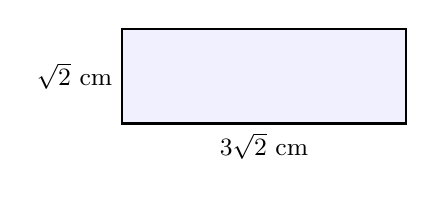
\begin{tikzpicture}[baseline=(current bounding box.north),scale=0.85]
  \draw[thick,fill=blue!6] (0,0) rectangle ({3*1.4142},1.4142);
  \node[below,font=\small] at ({1.5*1.4142},0) {$3\sqrt{2}$ cm};
  \node[left,font=\small] at (0,0.7071) {$\sqrt{2}$ cm};
\end{tikzpicture}

\vspace{8pt}
\raggedright
Perimeter $=3\sqrt{2}+\sqrt{2}+\ansline[1.1cm]+\ansline[1.1cm]$

\vspace{10pt}
\hspace*{4.9em}$=\ansline[1.8cm]$ cm
\end{minipage}\hfill
\begin{minipage}[t]{0.48\linewidth}
\raggedright
(b) The triangle has sides of length $2\sqrt{5}$ cm, $3\sqrt{5}$ cm and
$4\sqrt{5}$ cm. Work out its perimeter.

\vspace{4pt}
\centering
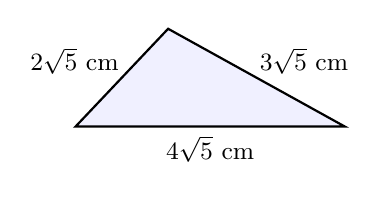
\begin{tikzpicture}[baseline=(current bounding box.north),scale=0.95]
  \draw[thick,fill=blue!6] (0,0) -- (3.6,0) -- (1.2375,1.3072) -- cycle;
  \node[below,font=\small] at (1.8,0) {$4\sqrt{5}$ cm};
  \node[above left,font=\small,inner sep=1pt] at (0.62,0.66) {$2\sqrt{5}$ cm};
  \node[above right,font=\small,inner sep=1pt] at (2.42,0.66) {$3\sqrt{5}$ cm};
\end{tikzpicture}

\vspace{4em}
\raggedright
Perimeter $=\ansline[1.8cm]$ cm
\end{minipage}

\vspace{1.5em}

\item \textbf{Harder.} In each of these the first surd is not a like surd
until it has been simplified. Simplify it using the formula from Part 2, then
collect like surds.
\begin{enumerate}
  \item Fill in the gaps: \quad
        $\sqrt{8}+\sqrt{2}=\gap\sqrt{2}+\sqrt{2}=\gap\sqrt{2}$
\end{enumerate}
\begin{multicols}{3}
\begin{enumerate}[resume]
  \item $\sqrt{12}+\sqrt{3}$
  \item $\sqrt{18}-\sqrt{2}$
  \item $\sqrt{45}+\sqrt{20}$
\end{enumerate}
\end{multicols}
\vspace{9em}

\end{enumerate}

\newpage

\parttitle{4}{Multiplying and dividing surds}

Part 2 showed that $\sqrt{18}=\sqrt{9}\times\sqrt{2}$. Read the other way
round, this says $\sqrt{9}\times\sqrt{2}=\sqrt{18}$: when we multiply two
square roots, we multiply the numbers under the roots. Dividing works in the
same way. Remember that $ab$ means $a\times b$.

\begin{formulas}{multiplying and dividing surds}
\renewcommand{\arraystretch}{1.95}%
\begin{tabular}{@{}>{\large}p{8.4cm}@{\hspace{1em}}l@{}}
$\sqrt{a}\times\sqrt{b}=\sqrt{ab}$ & for example \; $\sqrt{2}\times\sqrt{3}=\sqrt{6}$\\
$\sqrt{a}\div\sqrt{b}=\sqrt{a\div b}$ \; or \; $\dfrac{\sqrt{a}}{\sqrt{b}}=\sqrt{\dfrac{a}{b}}$
  & for example \; $\sqrt{15}\div\sqrt{3}=\sqrt{5}$\\
$\sqrt{a}\times\sqrt{a}=a$ & for example \; $\sqrt{7}\times\sqrt{7}=7$\\
$m\sqrt{a}\times n\sqrt{b}=mn\sqrt{ab}$ & for example \; $2\sqrt{3}\times4\sqrt{5}=8\sqrt{15}$\\
$m\sqrt{a}\div n\sqrt{b}=(m\div n)\sqrt{a\div b}$ & for example \; $8\sqrt{6}\div2\sqrt{3}=4\sqrt{2}$\\
\end{tabular}

\vspace{4pt}
In words: multiply or divide the numbers under the roots. Numbers in front are
multiplied or divided separately.
\end{formulas}

\begin{wex}{multiplying surds}
\small
\renewcommand{\arraystretch}{1.6}
\begin{tabular}{@{}l@{\hspace{2em}}l@{}}
$\sqrt{3}\times\sqrt{5}=\sqrt{3\times5}=\sqrt{15}$ & \\
$\sqrt{2}\times\sqrt{8}=\sqrt{2\times8}=\sqrt{16}=4$
  & the answer can be a whole number\\
$2\sqrt{3}\times4\sqrt{5}=(2\times4)\sqrt{3\times5}=8\sqrt{15}$
  & the numbers in front are multiplied separately\\
\end{tabular}
\end{wex}

\begin{enumerate}[resume]

\item Fill in the gaps in parts (a) and (b), then work out parts (c) to (j)
using the formulas. Some of the answers are whole numbers.
\begin{enumerate}
  \item $\sqrt{2}\times\sqrt{7}=\sqrt{\rootgap\times\rootgap}=\sqrt{\rootgap}$
  \item $3\sqrt{2}\times5\sqrt{7}=(\gap\times\gap)\sqrt{\rootgap\times\rootgap}
        =\ansline[1.6cm]$
\end{enumerate}
\vspace{4pt}
\begin{multicols}{4}
\begin{enumerate}[resume]
  \item $\sqrt{3}\times\sqrt{7}$
  \item $\sqrt{6}\times\sqrt{6}$
  \item $\sqrt{2}\times\sqrt{18}$
  \item $\sqrt{5}\times\sqrt{20}$
  \item $2\sqrt{5}\times3\sqrt{2}$
  \item $4\sqrt{3}\times2\sqrt{7}$
  \item $5\sqrt{2}\times\sqrt{3}$
  \item $3\sqrt{5}\times3\sqrt{5}$
\end{enumerate}
\end{multicols}

\end{enumerate}

\newpage

\begin{wex}{dividing surds}
\small
\renewcommand{\arraystretch}{1.6}
\begin{tabular}{@{}l@{\hspace{2em}}l@{}}
$\sqrt{15}\div\sqrt{3}=\sqrt{15\div3}=\sqrt{5}$ & \\
$\sqrt{50}\div\sqrt{2}=\sqrt{50\div2}=\sqrt{25}=5$
  & the answer can be a whole number\\
$8\sqrt{6}\div2\sqrt{3}=(8\div2)\sqrt{6\div3}=4\sqrt{2}$
  & the numbers in front are divided separately\\
\end{tabular}
\end{wex}

\begin{enumerate}[resume]

\item Fill in the gaps in parts (a) and (b), then work out parts (c) to (h)
using the formulas. Some of the answers are whole numbers.
\begin{enumerate}
  \item $\sqrt{21}\div\sqrt{7}=\sqrt{\rootgap\div\rootgap}=\sqrt{\rootgap}$
  \item $10\sqrt{15}\div5\sqrt{5}=(\gap\div\gap)\sqrt{\rootgap\div\rootgap}
        =\ansline[1.6cm]$
\end{enumerate}
\vspace{4pt}
\begin{multicols}{3}
\begin{enumerate}[resume]
  \item $\sqrt{30}\div\sqrt{6}$
  \item $\dfrac{\sqrt{22}}{\sqrt{2}}$
  \item $\dfrac{\sqrt{12}}{\sqrt{3}}$
  \item $\sqrt{63}\div\sqrt{7}$
  \item $8\sqrt{6}\div4\sqrt{2}$
  \item $12\sqrt{10}\div3\sqrt{2}$
\end{enumerate}
\end{multicols}
\vspace{10em}

\item The shapes are not drawn to scale. The area of a rectangle is its length
multiplied by its width.
\vspace{4pt}

\begin{minipage}[t]{0.32\linewidth}
(a) Fill in the gaps to find the area.

\vspace{4pt}
\centering
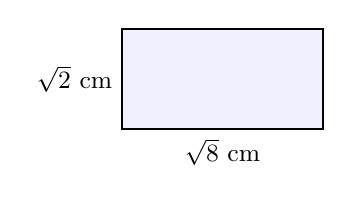
\begin{tikzpicture}[baseline=(current bounding box.north),scale=0.85]
  \draw[thick,fill=blue!6] (0,0) rectangle (3.0,1.5);
  \node[below,font=\small] at (1.5,0) {$\sqrt{8}$ cm};
  \node[left,font=\small] at (0,0.75) {$\sqrt{2}$ cm};
\end{tikzpicture}

\vspace{8pt}
\raggedright
Area $=\sqrt{2}\times\sqrt{8}$

\vspace{8pt}
\hspace*{2.4em}$=\sqrt{\rootgap}=\ansline[1cm]$ cm$^2$
\end{minipage}\hfill
\begin{minipage}[t]{0.32\linewidth}
(b) Work out the area.

\vspace{4pt}
\centering
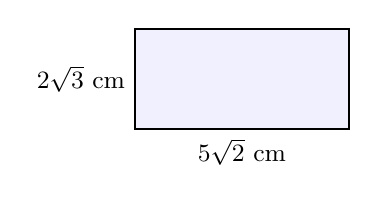
\begin{tikzpicture}[baseline=(current bounding box.north),scale=0.85]
  \draw[thick,fill=blue!6] (0,0) rectangle (3.2,1.5);
  \node[below,font=\small] at (1.6,0) {$5\sqrt{2}$ cm};
  \node[left,font=\small] at (0,0.75) {$2\sqrt{3}$ cm};
\end{tikzpicture}

\vspace{5em}
\raggedright
Area $=\ansline[2cm]$ cm$^2$
\end{minipage}\hfill
\begin{minipage}[t]{0.32\linewidth}
(c) The area is $\sqrt{35}$ cm$^2$. Work out the length.

\vspace{4pt}
\centering
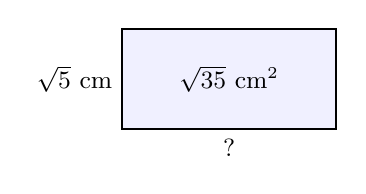
\begin{tikzpicture}[baseline=(current bounding box.north),scale=0.85]
  \draw[thick,fill=blue!6] (0,0) rectangle (3.2,1.5);
  \node[font=\small] at (1.6,0.75) {$\sqrt{35}$ cm$^2$};
  \node[below,font=\small] at (1.6,0) {$?$};
  \node[left,font=\small] at (0,0.75) {$\sqrt{5}$ cm};
\end{tikzpicture}

\vspace{5em}
\raggedright
Length $=\ansline[2cm]$ cm
\end{minipage}

\end{enumerate}

\newpage

\parttitle{5}{Many ways to make a surd}

Each box around a surd holds a calculation whose answer is that surd. Use the
formulas from this sheet, and check each box on your calculator. The first
diagram is done for you.

\begin{enumerate}[resume]

\item Complete each diagram.

\vspace{6pt}
\begin{minipage}[t]{0.5\linewidth}
\centering
\textbf{Example}\\[4pt]
\spider{$4\sqrt{3}$}{$\sqrt{3}+3\sqrt{3}$}{$6\sqrt{3}-2\sqrt{3}$}
  {$\sqrt{16}\times\sqrt{3}$}{$8\sqrt{6}\div2\sqrt{2}$}{$\sqrt{48}$}
\end{minipage}%
\begin{minipage}[t]{0.5\linewidth}
\centering
(a) Fill in the gaps.\\[4pt]
\spider{$5\sqrt{2}$}{$\sqrt{2}+\ansline[0.9cm]$}{$8\sqrt{2}-\gap\sqrt{2}$}
  {$\sqrt{\rootgap}\times\sqrt{2}$}{$10\sqrt{6}\div2\sqrt{\rootgap}$}{$\sqrt{\rootgap}$}
\end{minipage}

\vspace{16pt}
\begin{minipage}[t]{0.5\linewidth}
\centering
(b) Two boxes are done. Fill in the other three.\\[4pt]
\spider{$3\sqrt{5}$}{$\sqrt{5}+2\sqrt{5}$}{}{}{}{$\sqrt{45}$}
\end{minipage}%
\begin{minipage}[t]{0.5\linewidth}
\centering
(c) Fill in all five boxes.\\[4pt]
\spider{$6\sqrt{2}$}{}{}{}{}{}
\end{minipage}

\vspace{16pt}
\begin{minipage}[t]{0.5\linewidth}
\centering
(d) Fill in all five boxes.\\[4pt]
\spider{$2\sqrt{7}$}{}{}{}{}{}
\end{minipage}%
\begin{minipage}[t]{0.5\linewidth}
\centering
(e) Choose your own surd for the middle.\\[4pt]
\spider{}{}{}{}{}{}
\end{minipage}

\end{enumerate}

\newpage

\heading{Answers}

{\small
\begin{multicols}{2}
\raggedcolumns
\setlength{\parskip}{4pt}

\textbf{Q1.} $\sqrt{16}=4$, not a surd. \quad $\sqrt{2}=1.414213\ldots$, a
surd. \quad $\sqrt{49}=7$, not a surd. \quad $\sqrt{3}=1.732050\ldots$, a
surd. \quad $\sqrt{10}=3.162277\ldots$, a surd.

\textbf{Q2.} (a) 1.~$2.828427$ \quad 2.~$3.464101$ \quad 3.~$2.449489$ \quad
4.~$4.242640$ \quad 5.~$4.472135$ \quad 6.~$3.464101$ \quad 7.~$2.828427$
\quad 8.~$6.708203$ \quad 9.~$4.472135$ \quad 10.~$4.242640$ \quad
(b) $2\sqrt{2}=\sqrt{8}$, \; $\sqrt{12}=2\sqrt{3}$, \; $\sqrt{18}=3\sqrt{2}$,
\; $\sqrt{20}=2\sqrt{5}$. The numbers $\sqrt{6}$ and $3\sqrt{5}$ do not have
a partner.

\textbf{Q3.} (a) $\sqrt{4\times3}$; \; $\sqrt{4}\times\sqrt{3}$; \;
$2\times\sqrt{3}=2\sqrt{3}$ \quad (b) $\sqrt{25\times2}$; \;
$\sqrt{25}\times\sqrt{2}$; \; $5\times\sqrt{2}=5\sqrt{2}$ \quad
(c) $\sqrt{4\times6}=2\sqrt{6}$ \quad (d) $\sqrt{4\times7}=2\sqrt{7}$ \quad
(e) $\sqrt{9\times5}=3\sqrt{5}$ \quad (f) $\sqrt{9\times7}=3\sqrt{7}$ \quad
(g) $\sqrt{25\times3}=5\sqrt{3}$ \quad (h) $\sqrt{49\times2}=7\sqrt{2}$

\textbf{Q4.} (a) $6x$ \quad (b) $3y$ \quad (c) $4a$ \quad (d) $5m$ \quad
(e) $5x+2y$ \quad (f) cannot

\textbf{Q5.} (a) $(3+2)\sqrt{5}=5\sqrt{5}$ \quad
(b) $(9-4)\sqrt{7}=5\sqrt{7}$ \quad (c) $5\sqrt{2}$ \quad (d) $8\sqrt{6}$
\quad (e) $5\sqrt{11}$ \quad (f) $5\sqrt{5}$ \quad (g) $6\sqrt{3}$ \quad
(h) $7\sqrt{2}+3\sqrt{7}$ \quad (i) cannot: $\sqrt{2}$ and $\sqrt{3}$ are not
like surds \quad (j) $0$

\textbf{Q6.} (a) $3\sqrt{2}+\sqrt{2}+3\sqrt{2}+\sqrt{2}=8\sqrt{2}$ cm \quad
(b) $2\sqrt{5}+3\sqrt{5}+4\sqrt{5}=9\sqrt{5}$ cm

\textbf{Q7.} (a) $2\sqrt{2}+\sqrt{2}=3\sqrt{2}$ \quad
(b) $2\sqrt{3}+\sqrt{3}=3\sqrt{3}$ \quad
(c) $3\sqrt{2}-\sqrt{2}=2\sqrt{2}$ \quad
(d) $3\sqrt{5}+2\sqrt{5}=5\sqrt{5}$

\textbf{Q8.} (a) $\sqrt{2\times7}=\sqrt{14}$ \quad
(b) $(3\times5)\sqrt{2\times7}=15\sqrt{14}$ \quad (c) $\sqrt{21}$ \quad
(d) $6$ \quad (e) $\sqrt{36}=6$ \quad (f) $\sqrt{100}=10$ \quad
(g) $6\sqrt{10}$ \quad (h) $8\sqrt{21}$ \quad (i) $5\sqrt{6}$ \quad
(j) $9\times5=45$

\textbf{Q9.} (a) $\sqrt{21\div7}=\sqrt{3}$ \quad
(b) $(10\div5)\sqrt{15\div5}=2\sqrt{3}$ \quad (c) $\sqrt{5}$ \quad
(d) $\sqrt{11}$ \quad (e) $\sqrt{4}=2$ \quad (f) $\sqrt{9}=3$ \quad
(g) $2\sqrt{3}$ \quad (h) $4\sqrt{5}$

\textbf{Q10.} (a) $\sqrt{16}=4$ cm$^2$ \quad
(b) $2\sqrt{3}\times5\sqrt{2}=10\sqrt{6}$ cm$^2$ \quad
(c) $\sqrt{35}\div\sqrt{5}=\sqrt{7}$ cm

\textbf{Q11.} (a) $\sqrt{2}+4\sqrt{2}$; \; $8\sqrt{2}-3\sqrt{2}$; \;
$\sqrt{25}\times\sqrt{2}$; \; $10\sqrt{6}\div2\sqrt{3}$; \; $\sqrt{50}$.
\quad Parts (b) to (e) have many answers. For example:
(b) $4\sqrt{5}-\sqrt{5}$; \; $\sqrt{9}\times\sqrt{5}$; \;
$6\sqrt{10}\div2\sqrt{2}$. \quad
(c) $2\sqrt{2}+4\sqrt{2}$; \; $7\sqrt{2}-\sqrt{2}$; \;
$\sqrt{36}\times\sqrt{2}$; \; $12\sqrt{6}\div2\sqrt{3}$; \; $\sqrt{72}$.
\quad
(d) $\sqrt{7}+\sqrt{7}$; \; $5\sqrt{7}-3\sqrt{7}$; \;
$\sqrt{4}\times\sqrt{7}$; \; $6\sqrt{14}\div3\sqrt{2}$; \; $\sqrt{28}$.
\quad (e) Any surd, with five calculations that give it.

\end{multicols}
}

\end{document}
